\chapter{実装}
\label{make}
\section{ハードウェア}
提案手法に用いる圧力センサを搭載したヘルメットを実装した.このデバイスの構成を図\ref{device},プロトタイプデバイスの全体図を図\ref{met_over}に示す.センサ値を正しく取得するには,センサとヘルメット装着者の頭部が密着している必要がある.そのため,フルフェイス型のB\&B社製BB100フルフェイスヘルメットを用いた.実装したプロトタイプデバイスの内部を図\ref{met_in}に示す.今回用いたヘルメットはフリーサイズであり,また内装の脱着が困難であった.そのため,頭頂部の内装を取り外して,新たに厚みのあるウレタンスポンジを取り付けた.図\ref{sensor}のようにウレタンスポンジの中央部に切り込みを入れ,インターリンク エレクトロニクス社製のFSR402,FSR402 ShortTailを挿し込むことで圧力センサを実装した.この圧力センサは頭頂部に4個,頭頂部周囲に16個,後頭部に6個,左右チークパッド部に6個の合計32個を搭載した.配線はヘルメットの頭頂部にドリルで穴あけ加工をし,ヘルメット外部に取り付けた10KΩの抵抗を配線してあるプリント基板を経由して,Arduino MEGA2560 R3の5V電源,GND,アナログ入力ポートに接続した.センサ1つあたりの回路図を図\ref{circuit}に示す.図\ref{circuit}に示した回路を図\ref{print}のプリント基板を通して32個並列に接続した.このプリント基板は取り外しが可能かつしっかりと固定するため,ヘルメットのシールド固定用に開けられたネジ穴を流用し,左頬部分にボルトで固定している.

\begin{figure}[!t]
  \begin{center}
    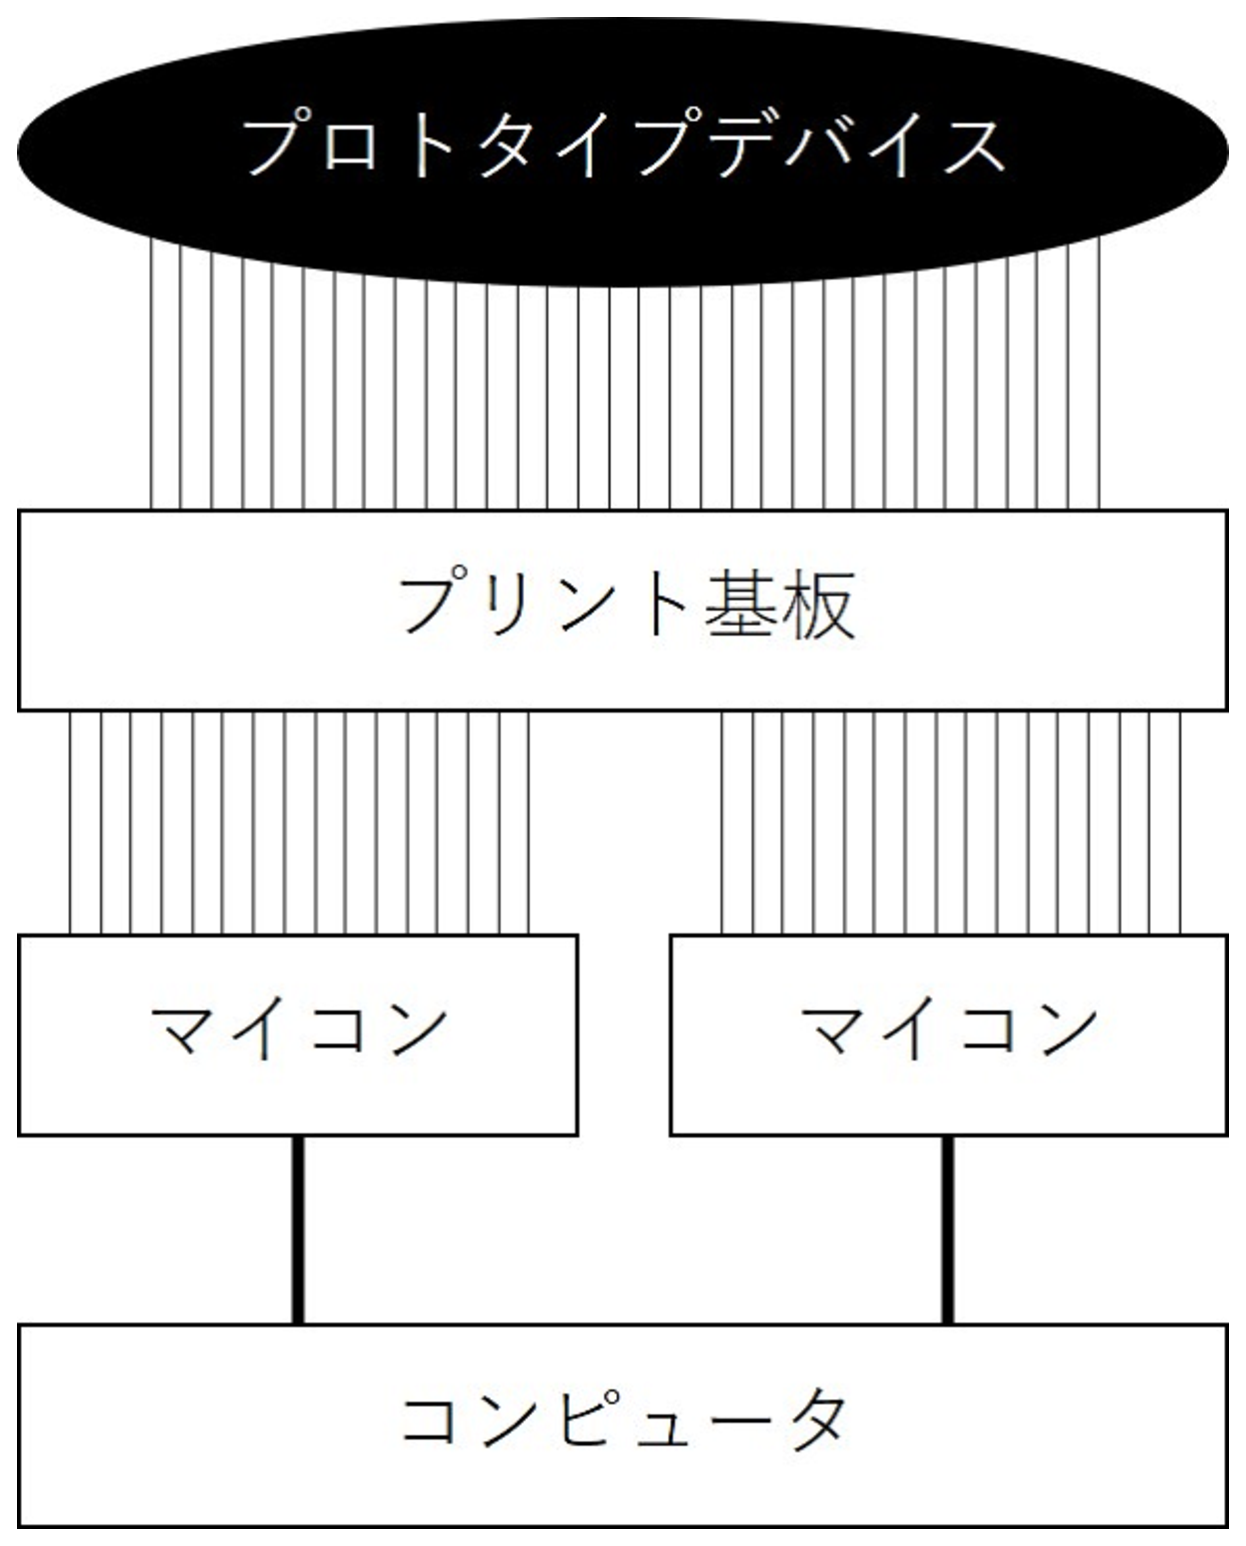
\includegraphics[width=0.5\linewidth]{figure/device.eps}
  \end{center}
  \caption{デバイス構成}
  \label{device}
\end{figure}

\begin{figure}[!t]
  \begin{center}
    \includegraphics[width=0.5\linewidth]{figure/met_over.eps}
  \end{center}
  \caption{プロトタイプデバイスの全体図}
  \label{met_over}
\end{figure}

\begin{figure}[!t]
  \begin{center}
    \includegraphics[width=0.5\linewidth]{figure/met_in.eps}
  \end{center}
  \caption{プロトタイプデバイスの内部}
  \label{met_in}
\end{figure}

\begin{figure}[!t]
  \begin{center}
    \includegraphics[width=0.5\linewidth]{figure/sensor.eps}
  \end{center}
  \caption{センサの実装方法}
  \label{sensor}
\end{figure}

\begin{figure}[!t]
  \begin{center}
    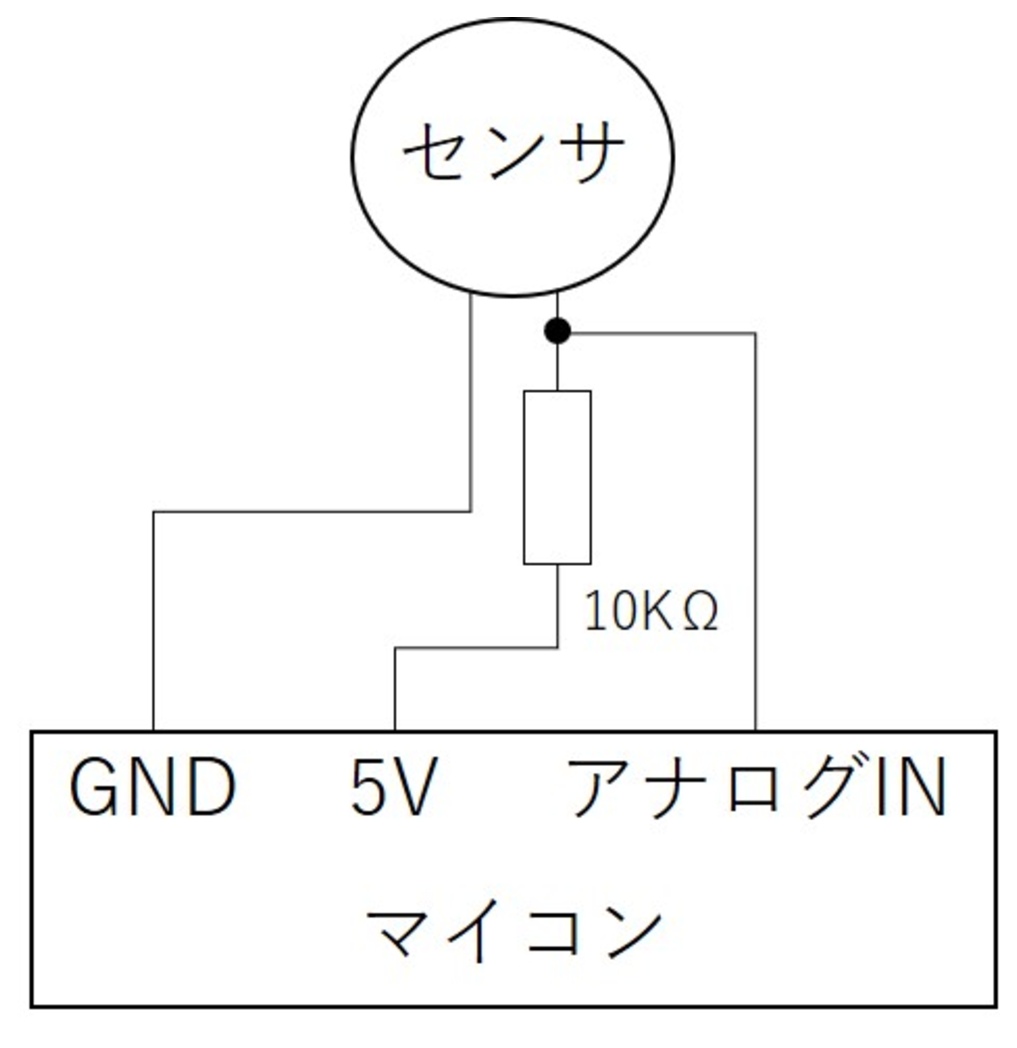
\includegraphics[width=0.5\linewidth]{figure/circuit.eps}
  \end{center}
  \caption{センサ1つあたりの回路図}
  \label{circuit}
\end{figure}

\begin{figure}[!t]
  \begin{center}
    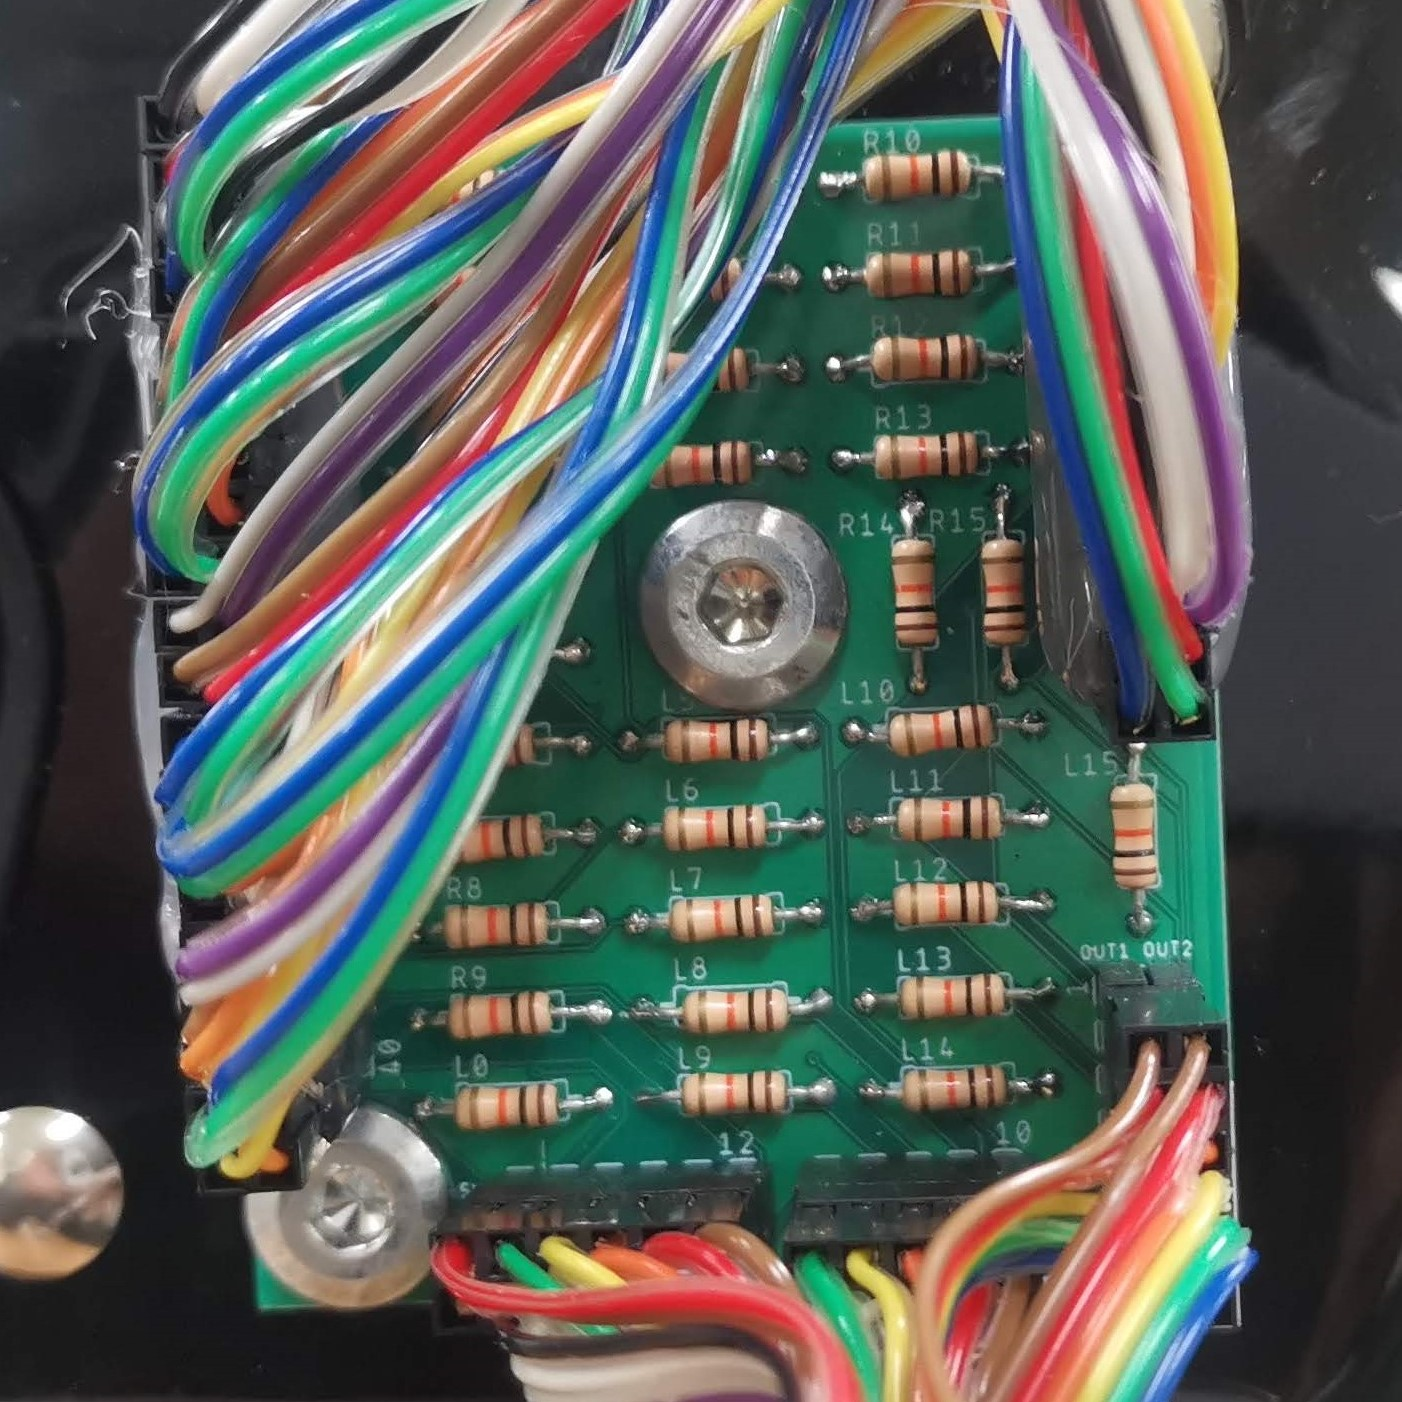
\includegraphics[width=0.5\linewidth]{figure/print.eps}
  \end{center}
  \caption{プリント基板}
  \label{print}
\end{figure}

\section{ソフトウェア}
データの収集にはArduinoIDEを用いてマイコンを制御し,Pythonでセンサデータをコンピュータ上にcsvとして収集するプログラムを作成した.次にデータの解析はPython上でcsvを読み出し,sklearn.covariance.MinCovDetを用いてマハラノビス距離を計算した.そして,計算結果に対し閾値を移動させながら比較,識別しながら評価指標を計算するプログラムを実装した.\par
ここで用いたsklearn.covariance.MinCovDetとは,異常値に対して頑健な共分散行列の推定アルゴリズムであるMinimum Covariance Determinant(以下MCDと表記)を高速化したFast-MCD\cite{fast_mcd}を実装したscikit-learnのライブラリである.